\hl{As we mentioned before, we use the transfer learning method to learn the self-defined categories. In this section, we review some problems transfer learning faces and the popular methods to learn new categories in transfer learning.} 
\begin{figure}
	\centering
	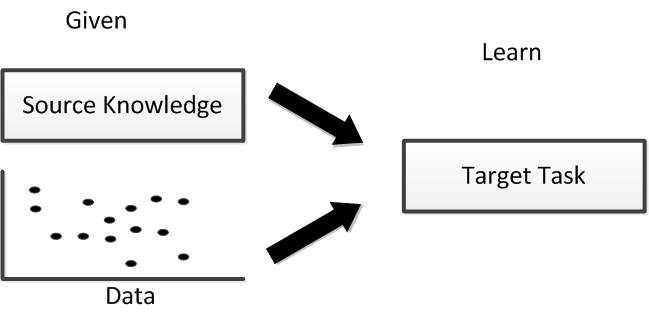
\includegraphics[scale =.7]{relatedwork/fig/transfer.png}
	\caption{Apart from the standard machine learning, transfer learning can leverage the information from an additional source: knoweldge from one or more related tasks.}
\end{figure}

Traditional machine learning algorithms try to build the classifiers from a set of training data and apply to the test data with the same distribution to the training data. In contrast, transfer learning attempts to change this by transfer the learned knowledge from one or several tasks (called source tasks) to improve a related new task (called target task).

Transfer learning can be categorized into 3 sub-settings: \textit{inductive transfer learning, transductive transfer leanring} and \textit{unsupervised transfer learning} based on the different situations of the source and target domains and tasks. \cite{pan2010survey}. We compared the differences of these three sub-categories and show them in Table \ref{tab:related:transfersetting}. \hl{Recalling our learning} self-defined category problem, we already obtained the source models from labelled source data and our goal is to utilize the knowledge from the source models and help us to train the models from a small set of labelled examples, i.e. examples from our self-defined categories. From Table \ref{tab:related:transfercmp} and \ref{tab:related:transfersetting} we can see that, our problem should be classified as inductive transfer learning. More specifically, it belongs to the multi-task transfer learning.

\begin{table}[htbp]
	\centering
	\caption{Relationship between traditional machine learning and different transfer learning settings}
	\begin{tabular}{|c|c|c|c|}
		\hline
		\multicolumn{2}{|c|}{Learning settings} & Source target domain & Source target task \\
		\hline
		\multicolumn{2}{|c|}{Traditional machine learning} & the same & the same \\\hline
		\multirow{3}{*}{Transfer learning} & Inductive transfer learning & the same & different but related \\\cline{2-4}
		& Unsupervised transfer learning & different but related & different but related \\\cline{2-4}
		& Transductive transfer learning & different but related & the same \\\hline	
	\end{tabular}%
	\label{tab:related:transfercmp}%
\end{table}%

\begin{table}[htbp]
	\centering
	\caption{Various settings of transfer learning}
	\begin{tabular}{|c|C{4cm}|c|c|}
		\hline
		& Related areas & Source data & Target data \\
		\hline
		\multirow{2}[4]{*}{Inductive transfer learning} & self-taught learning & unlabeled & labeled \\\cline{2-4}
		& multi-task learning & labeled & labeled \\\hline
		 Transductive transfer learning& domain adaptation, Sample selection bias & labeled & unlabeled \\\hline
		Unsupervised transfer learning &       & unlabeled & unlabeled \\
		\hline
	\end{tabular}%
	\label{tab:related:transfersetting}%
\end{table}%
\subsection{Inductive Transfer Learning}
In inductive transfer learning, we try to utilize the knowledge from the source task to help learning the target task. Here we give a formal definition of inductive transfer learning \cite{pan2010survey}:
\begin{definition}{\textbf{(Inductive Transfer Learning)}}
	Given a source domain $D_s$ and the source learning task $T_s$, a target domian $D_t$ and the target learning task $T_t$, inductive transfer learning aims to help improve the learning of the target task function $f_t(\cdot)$ in $D_t$ using the knowledge from $D_s$ and $T_s$ where $T_s \neq T_t$.
\end{definition}

According to the type of the source knowledge comes from, inductive transfer learning can be split into 3 major streams: instance transfer, feature representation transfer and parameter transfer.

The core idea of instance transfer learning is to select some useful data from the source task to help learning the target task. Dai et al. \cite{dai2007boosting} propose a method (called TrAdaBoost) that can select the most useful examples from the source task as the additional training examples for the target task. These useful examples are iteratively re-weighted according to the classification results of some base classifiers. Jiang et al. \cite{jiang2007instance} propose a method that can ignore the "misleading" examples from the source data based on the conditional probabilities on the source task $P(y_t|x_t)$ and target task $P(y_s|x_s)$. Liao et al. \cite{liao2005logistic} propose a active learning method that selects and labels the unlabeled data from the target data with the help of the source data. Ben-David et al. \cite{ben2010theory} provide a theoretical analysis the lowest target test error for different source data combination strategies when the source data is large and target training set is small.   

Feature representation transfer aims to find a good feature representations to reduce the gap between the source and target domains.According to the size of labeled examples in the source data, feature representation transfer consists of two approaches: supervised feature construction and unsupervised feature construction. When the source data are labeled, supervised feature transfer learning is used to find the feature representations shared in related tasks to reduce the difference between the source and target tasks. Evgeniou et al. \cite{evgeniou2007multi} propose a method that can learn sparse low-dimension feature representations that can share between different tasks. Jie et al. \cite{jie2011multiclass} reconstruct the feature representations for the target data by using the outputs of the source models as the auxiliary feature representations. In unsupervised feature representation transfer learning, Daume III \cite{daume2009frustratingly} proposes a simple feature reconstruction method for both source and target data so that source and target data are triple argumented and a SVM model is trained on both source and target data.

Parameter transfer assumes that there should be some parameters or prior distribution of the hyperparameters in the individual models of related tasks. Most of the approaches are designed under the multi-task learning scenario. Therefore, in this thesis, we also focus on the parameter transfer approach to leverage the knowledge from the source data. In parameter transfer learning, there are three major frameworks: a regularization framework, a Bayesian framework and a neural network framework.
\begin{figure}
	\centering
	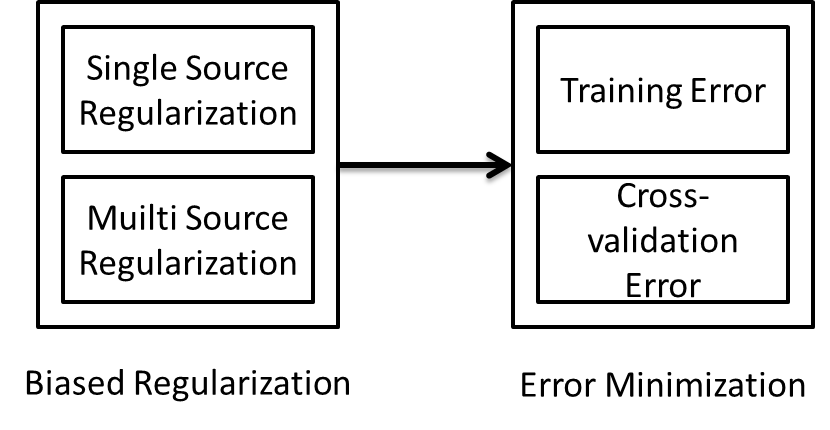
\includegraphics[scale =1]{relatedwork/fig/parameters.png}
	\caption{Two steps for parameter transfer learning. In the first step multi-source and single source combination are usually used to generate the regularazation term. The hyperplane for the transfer model can be obtained by either minimizing training error or cross-validation error on the target training data.}
\end{figure}
\begin{itemize}
	\item Regularization framework: In the regularization framework, some researchers propose to transfer the parameters of the SVM following the assumption that the hyperplane for the target task should be related to the hyperplane of the source models. Evgeniou et al. \cite{evgeniou2004regularized} propose an idea that the hyperplane of the SVM for the target task should be separate into two terms: a common term shared over tasks and a specific term related to the individual task. Inspired by this idea, some researchers propose different strategies to combine these two terms for transfer learning \cite{aytar2011tabula} \cite{tommasi2010safety} \cite{yang2007cross}. Most of these work contains two steps. In the first step, a SVM objective function with a biased regularization term for the target model is build. Then another objective function is build to reduce the empirical error of the target model on the target data.
	\item Neural network framework. In neural network framework, the idea is to use the parameters of a CNN pre-trained from a very large dataset as an initialization to reduce the bias when the target data is small. Yosinski et al. \cite{yosinski2014transferable} show that the high level layer parameters are more related to a specific task while the low level layer ones are more general and transferable. This framework is widely used for image recognition task. By re-using and fine-tuning the parameters of some layers in the pre-trained model, the bias of the target task can be greatly alleviated \cite{Chatfield14} \cite{hoffman2013one}  \cite{zeiler2014visualizing} \cite{NIPS2014_Zhou}. 
	\item Bayesian framework. In Bayesian framework, one or several posterior probabilities of the source data or parameters of the source model can be used to generate a prior probability for the target task. With this prior probability, a posterior probability for the target task can be obtained with the target data.
	Li et al. \cite{fei2006one} use a prior probability density function to model the knowledge from the source and modify it with the data from target to generate posterior density for detection and recognition. 
	Rosenstein et al. \cite{rosenstein2005transfer} use hierarchical Bayesian method to estimate the posterior distribution for all the parameters and the overall model can decide the similarities of the source and target tasks. 
\end{itemize}


\subsection{Avoid Negative Transfer}
In transfer learning, for a given target task, the performance of a transfer method depends on two aspects: the quality of the source task and the transfer ability of the transfer algorithm. The quality of the source task refers to how the source and target tasks are related. If there exists a strong relationship between the source and target, with a proper transfer method, the performance in the target task can be significantly improved. However, if the source and target tasks are not sufficiently related, despite of the transfer ability of the transfer algorithm, the performance in the target task may fail to be improved or even decrease. In transfer learning, negative transfer refers to the degraded performance compare to a method without using any knowledge from the source \cite{pan2010survey}. 
For example, we can use a teacher-student diagram to illustrate the procedure of transfer learning. The student (target model) would like to learn the new knowledge (target task) with the assistance of a teacher (source knowledge). If the teacher can provide helpful knowledge (related knowledge), the student can learn the new knowledge very quickly (positive transfer). If the teacher can only provide useless knowledge, the student could not learn the new knowledge effectively or even get confused (negative transfer).

\begin{figure}
\centering
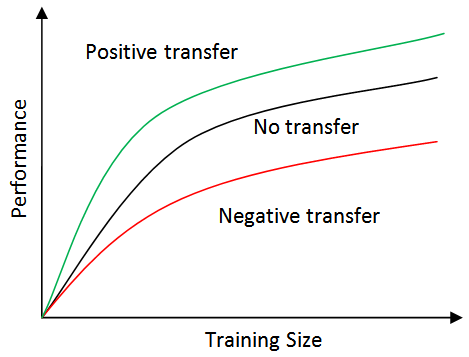
\includegraphics[scale=.7]{relatedwork/fig/negative.png}
\caption{Positive transfer VS Negative transfer.}
\end{figure}

Another important aspect that affect the learning performance is the transfer ability of the algorithm used for the target task. An ideal transfer algorithm would be able to produce positive transfer on related tasks while avoiding negative transfer on unrelated tasks. However, in practice, it is not easy to achieve these two goals simultaneously. Approaches that can avoid negative transfer often bring some affects on positive transfer due to their caution. On the other hand, approaches using aggressive transfer strategies often have little or no protection against negative transfer \cite{torrey2009transfer}. Even though voiding negative transfer is an important issue in transfer learning, how to avoid negative transfer has not been widely addressed \cite{lu2015transfer} \cite{pan2010survey}. Previous work show suggest that negative transfer can be alleviated through 3 approaches \cite{torrey2009transfer}: 
\begin{itemize}
	\item Rejecting unrelated source information. A important approach to avoid negative transfer is to recognize and reject unrelated and harmful source knowledge. The goal of this approach is to minimize the impact of the unrelated source, so that the transfer model performs no worse than the learned model without transfer. Therefore, in some extreme situation, the transfer model is allowed to completely ignore the source knowledge. 
		Torrey et al. \cite{torrey2005using} propose a method using advice-taking algorithm to reject the unrelated source knowledge. 
		Rosenstein et al. \cite{rosenstein2005transfer} present an approach that use naive Bayes classifier to detect and reject the unrelated source.
	\item Choosing correct source task. When the source knowledge come from more than one candidate source, it is possible for the transfer model to select the best source knowledge of the candidates. In this scenario, leverage the knowledge from the best candidate may be effective against negative transfer as long as the best source knowledge is sufficiently related. 
		Talvitie et al. \cite{talvitie2007experts} propose a method that can iteratively evaluate the candidate sources through a trail-and-error approach and select the best one to transfer. Kuhlmann et al. \cite{kuhlmann2007graph} construct a kernel function from certain sources for the target task by estimating the bias from a set of candidate sources whose relationship to the target task is unknown.
	\item Measuring task similarity. To achieve a better transfer performance, it is reasonable for a transfer method to transfer the knowledge from multiple sources instead of just choosing a single source. In this approach, some methods try to involve all the source knowledge without considering the explicit relationship between the source and target. The other methods try to model the relationships between the source and target tasks and use the information as a part of their transfer methods which can significantly reduce the affect of negative transfer.
		 Bakker et al. \cite{bakker2003task} propose a method to provide guidance on how to avoid negative transfer by using clustering and Bayesian approach to estimate the similarities between the target task and multiple source tasks.
		 Tommasi et al. \cite{tommasi2014learning} construct the transfer model by using some transfer parameters to measure the relationships between each source and the target tasks and the transfer parameters are optimized by minimizing the cross-validation error of the transfer model. Similar approaches can be found in \cite{jie2011multiclass} \cite{kuzborskij2013n}.
		 Kuzborskij et al. \cite{kuzborskij2013stability} provide some theoretical analysis of transfer learning and show that regularized least square SVM with truncation function and leave-one-out cross-validation for source task measurement can reduce negative transfer even though the training data of the target task is relatively small.
\end{itemize}

Here we can see that most of the previous approaches focus on measuring the similarity of the source and target tasks, i.e. try to assign the most related source tasks to the target one through various of metrics and use aggressive transfer algorithm to exploit the source knowledge. Just a few work \cite{tommasi2010safety} \cite{kuzborskij2013stability} addressed the problem that a sophisticated transfer algorithm should be designed to better exploit the source knowledge as well as avoid negative transfer. Therefore, in this thesis, we mainly focus on how to design a better transfer algorithm for transfer learning while certain source knowledge is assigned. 

To summarize, in this section, we reviewed 3 types of inductive transfer learning approaches and discussed how to avoid the negative transfer in transfer learning. In our problem, as we have the assumption that the source data is access prohibited, we are not able to use instance transfer and feature transfer approaches. Therefore, we propose a transfer method based on parameter transfer approach. To reduce the affect negative transfer, in our transfer method, we adopt several ideas from the work mentioned above. 


